%%%%%%%%%%%%%%%%%%%%%%%%%%%%%%%%%%%%%%%%%%%%%%%%%%%%%%%%%%%%%%%%%%%%%
%
% CSCI 1430 Written Question Template
%
% This is a LaTeX document. LaTeX is a markup language for producing 
% documents. Your task is to fill out this document, then to compile 
% it into a PDF document. 
% You will then upload this PDF to `Gradescope' - the grading system 
% that we will use. Instructions for upload will follow soon.
%
% 
% TO COMPILE:
% > pdflatex thisfile.tex
%
% If you do not have LaTeX and need a LaTeX distribution:
% - Online Tool: https://www.overleaf.com/ (recommended)
% - Departmental machines have one installed.
% - Personal laptops (all common OS): www.latex-project.org/get/
%
% If you need help with LaTeX, please come to office hours. 
% Or, there is plenty of help online:
% https://en.wikibooks.org/wiki/LaTeX
%
% Good luck!
% James and the 1430 staff
%
%%%%%%%%%%%%%%%%%%%%%%%%%%%%%%%%%%%%%%%%%%%%%%%%%%%%%%%%%%%%%%%%%%%%%

\documentclass[11pt]{article}

\usepackage[english]{babel}
\usepackage[utf8]{inputenc}
\usepackage[colorlinks = true,
            linkcolor = blue,
            urlcolor  = blue]{hyperref}
\usepackage[a4paper,margin=1.5in]{geometry}
\usepackage{stackengine,graphicx}
\usepackage{fancyhdr}
\setlength{\headheight}{15pt}
\usepackage{microtype}
\usepackage{times}
% a great python code format: https://github.com/olivierverdier/python-latex-highlighting
\usepackage{pythonhighlight}

\frenchspacing
\setlength{\parindent}{0cm} % Default is 15pt.
\setlength{\parskip}{0.3cm plus1mm minus1mm}

\pagestyle{fancy}
\fancyhf{}
\lhead{Project 0 Questions}
\rhead{CSCI 1430}
\rfoot{\thepage}

\date{}

\title{\vspace{-1cm}Project 0 Questions}


\begin{document}
\maketitle
\vspace{-2cm}
\thispagestyle{fancy}

\section*{Instructions}
\begin{itemize}
  \item Compile and read through the included Python tutorial.
  \item 3 questions.
  \item Include code.
  \item Feel free to include images or equations.
  \item Please make this document anonymous.
  \item \textbf{Please use only the space provided and keep the page breaks.} Please do not make new pages, nor remove pages. The document is a template to help grading.
  \item If you really need extra space, please use new pages at the end of the document and refer us to it in your answers.
\end{itemize}

\section*{Questions}

\paragraph{Q1:} Please find and read the course collaboration policy on the \href{http://cs.brown.edu/courses/csci1430/}{course website}, and write a paraphrased version.

%%%%%%%%%%%%%%%%%%%%%%%%%%%%%%%%%%%
\paragraph{A1:} Your answer here.



%%%%%%%%%%%%%%%%%%%%%%%%%%%%%%%%%%%

% Please leave the pagebreak
\pagebreak
\paragraph{Q2:} We wish to set all pixels that have a value of 10 or less to 0, to remove camera sensor noise. However, our code is slow when run on a database with 1000 grayscale images.

\emph{Image:} \href{grizzlypeakg.png}{grizzlypeakg.png}

\begin{python}
from skimage import io

A = io.imread('grizzlypeakg.png')
(m1,n1) = A.shape
for i in range(m1):
    for j in range(n1):
        if A[i,j] <= 10 :
            A[i,j] = 0       
\end{python}

\paragraph{Q2.1:} How could we speed it up? Please include your code.

%%%%%%%%%%%%%%%%%%%%%%%%%%%%%%%%%%%
\paragraph{A2.1:} Your answer here.



%%%%%%%%%%%%%%%%%%%%%%%%%%%%%%%%%%%

% Please leave the pagebreak
\pagebreak
\paragraph{Q2.2:} What factor speedup would we receive over 1000 images? Please measure it and include your code.

Ignore file loading; assume all images are equal resolution; don't assume that the time taken for one image $\times1000$ will equal $1000$ image computations, as single short tasks on multitasking computers often take variable time.

\emph{Note: We found that running the slow code on 1000 images might take 45 minutes or more! You can compute the factor on just 10 images. For the sped-up version, you might need to compute the time on more images to receive a more reliable estimate of the average time. Be sure to compensate for the number of images computed against in your speedup factor.}

%%%%%%%%%%%%%%%%%%%%%%%%%%%%%%%%%%%
\paragraph{A2.2:} Your answer here.



%%%%%%%%%%%%%%%%%%%%%%%%%%%%%%%%%%%

% Please leave the pagebreak
\pagebreak
\paragraph{Q2.3:} Next, we wish to operate on color images. How does your speeded-up version from Q2.2 change for color images? Please implement and measure it, report the speed factor change, and include your code.

\emph{Note: We will change the value in each color channel; we do not wish to convert the image to grayscale.}

\emph{Image:} \href{grizzlypeak.jpg}{grizzlypeak.jpg}

%%%%%%%%%%%%%%%%%%%%%%%%%%%%%%%%%%%
\paragraph{A2.3:} Your answer here.



%%%%%%%%%%%%%%%%%%%%%%%%%%%%%%%%%%%

% Please leave the pagebreak
\pagebreak
\paragraph{Q3:} We wish to reduce the brightness of an image by editing the values in its matrix. But, when trying to visualize the result, we see some ``errors''.

\emph{Image:} \href{gigi.jpg}{gigi.jpg}

\begin{python}
from skimage import io
import matplotlib.pyplot as plt
import numpy as np

I =  io.imread('gigi.jpg').astype(np.float32)
I = I - 50
plt.imshow( I )
plt.show()
\end{python}

\paragraph{Q3.1:} What is incorrect with this approach? How can it be fixed while maintaining the same intended brightness reduction? Please include your code and result image.

%%%%%%%%%%%%%%%%%%%%%%%%%%%%%%%%%%%
\paragraph{A3.1:} Your answer here.

% Example image inclusion; replace with your result image:
% 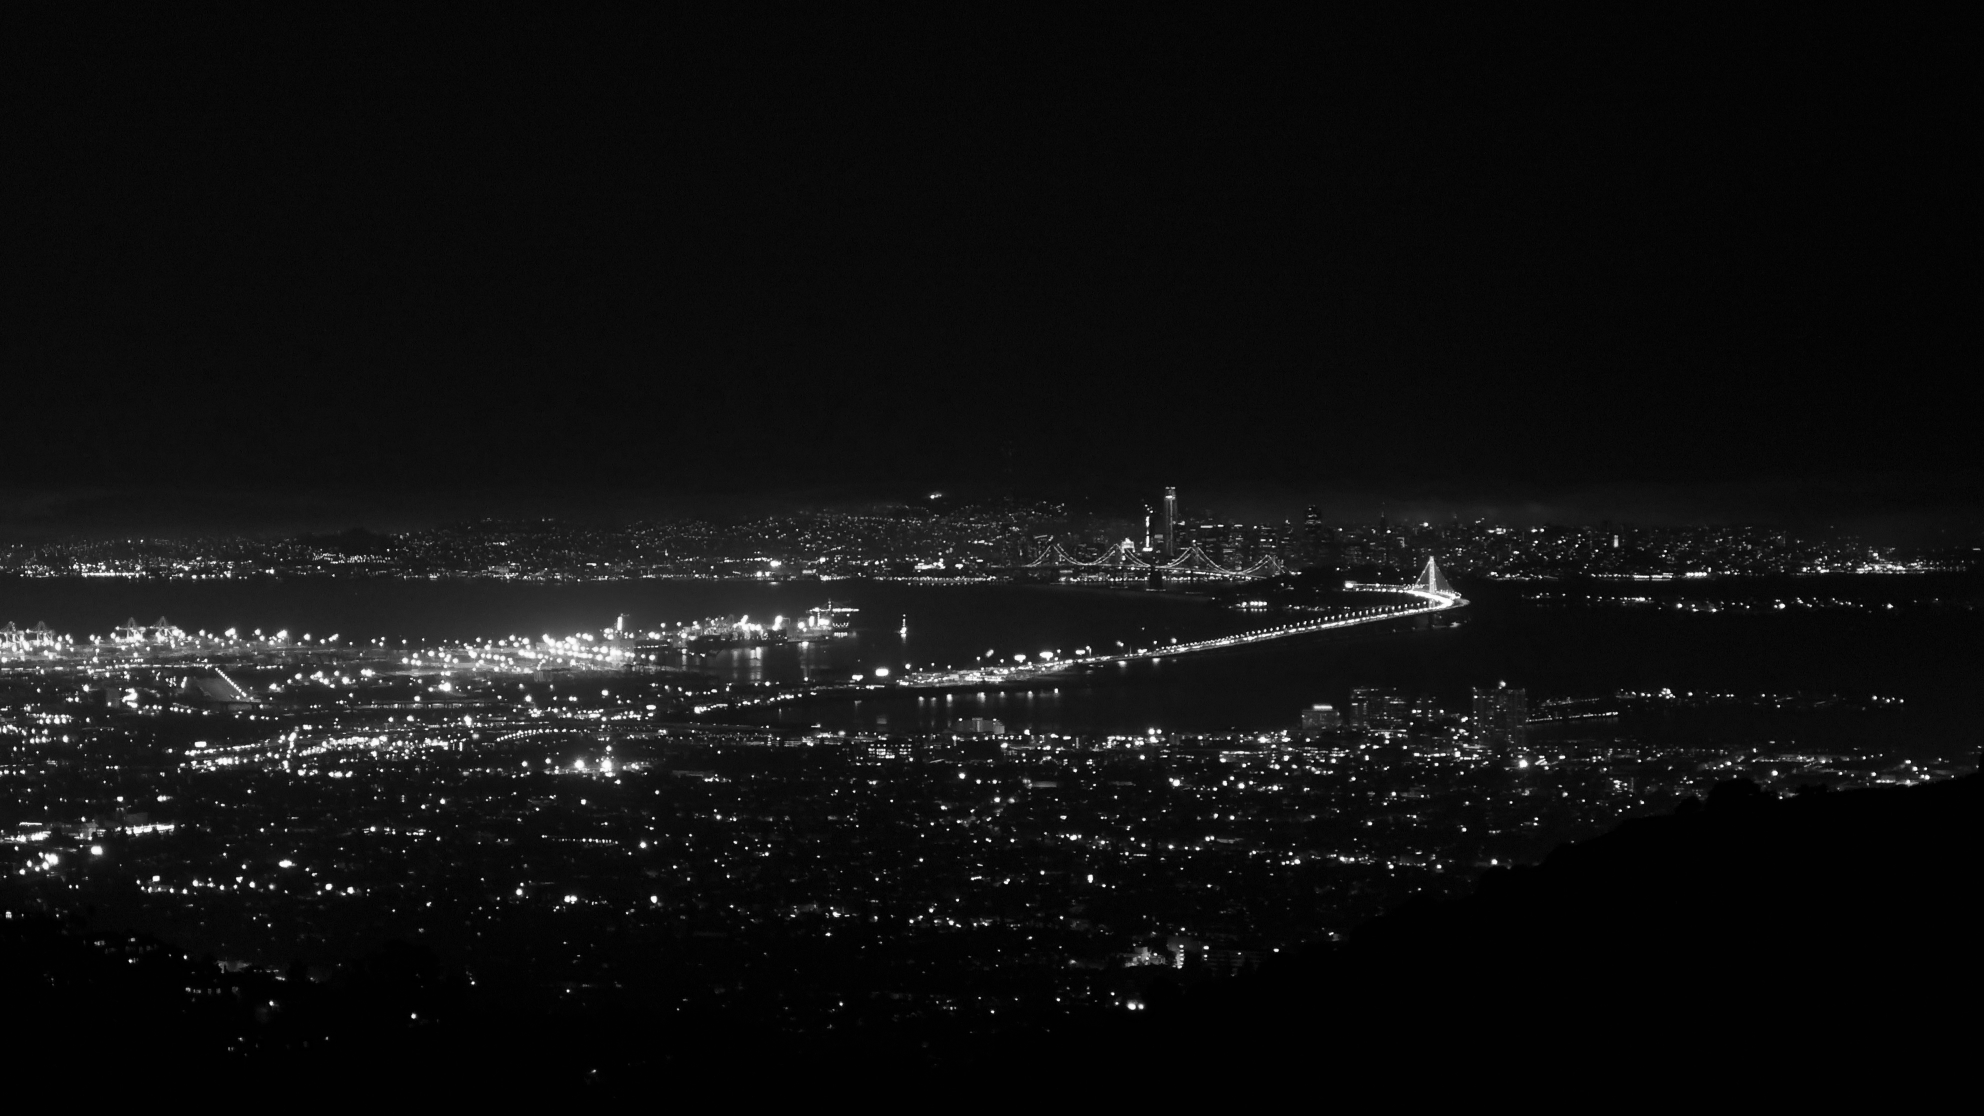
\includegraphics[width=\textwidth]{grizzlypeakg.png}




%%%%%%%%%%%%%%%%%%%%%%%%%%%%%%%%%%%

\end{document}
